\documentclass{beamer}
\usepackage{graphicx}
\title{Design, Validation and Prototype of  AI accelerator system-on-chip using the AHIR-V2 toolset}
\author{Aman Dhammani, Harshad Ugale, Madhav P. Desai \\ Department of Electrical Engineering, IIT Bombay \\ email: madhav@ee.iitb.ac.in}
\begin{document}
\maketitle

\frame{\frametitle{Overview}
\begin{itemize}
\item Designed and validated an entire system-on-chip with an AI/ML accelerator.
\begin{itemize}
\item AI/ML inference engine: UNET.
\item Embedded processor: AJIT 1x1x32 core.
\item 100Mbps Ethernet interface.
\end{itemize}
\item Hardware cost has been characterized.
\item Performance has been characterized.
\end{itemize}

}

\frame{\frametitle{System-on-chip block diagram}

\begin{figure}
\centering
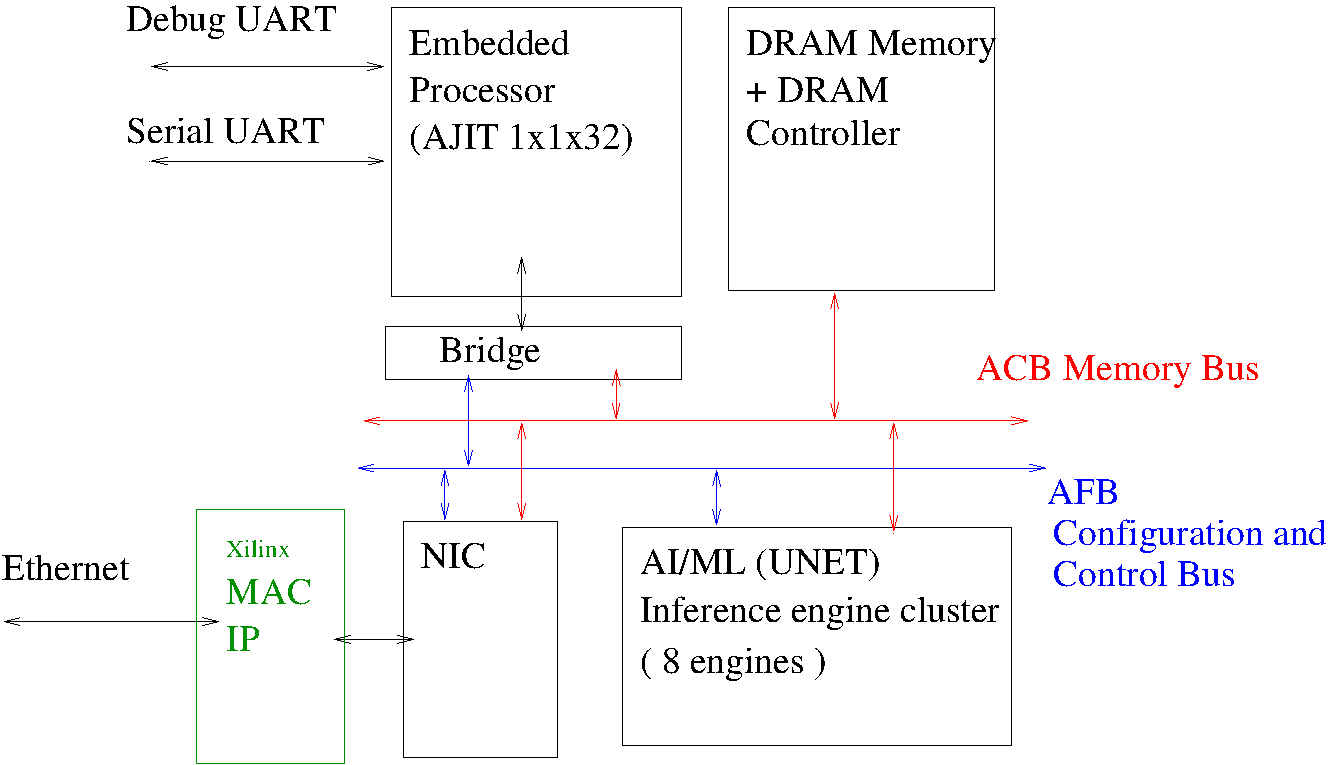
\includegraphics[width=10cm]{figs/BlockDiagram.pdf}
\caption{The system on chip: all blocks designed by our team using AHIR-V2, except for Xilinx Ethernet MAC}
\label{fig:BlockDiagram}
\end{figure}

}

\frame[containsverbatim]{\frametitle{System-on-chip execution flow}
\begin{verbatim}
download processor driver code
download UNET parameters/weights
jump to processor driver

processor driver:
  download image
  apply UNET stages 
  upload segmented image
\end{verbatim}
}

\frame[containsverbatim]{\frametitle{UNET hardware implementation}
\begin{figure}
\centering
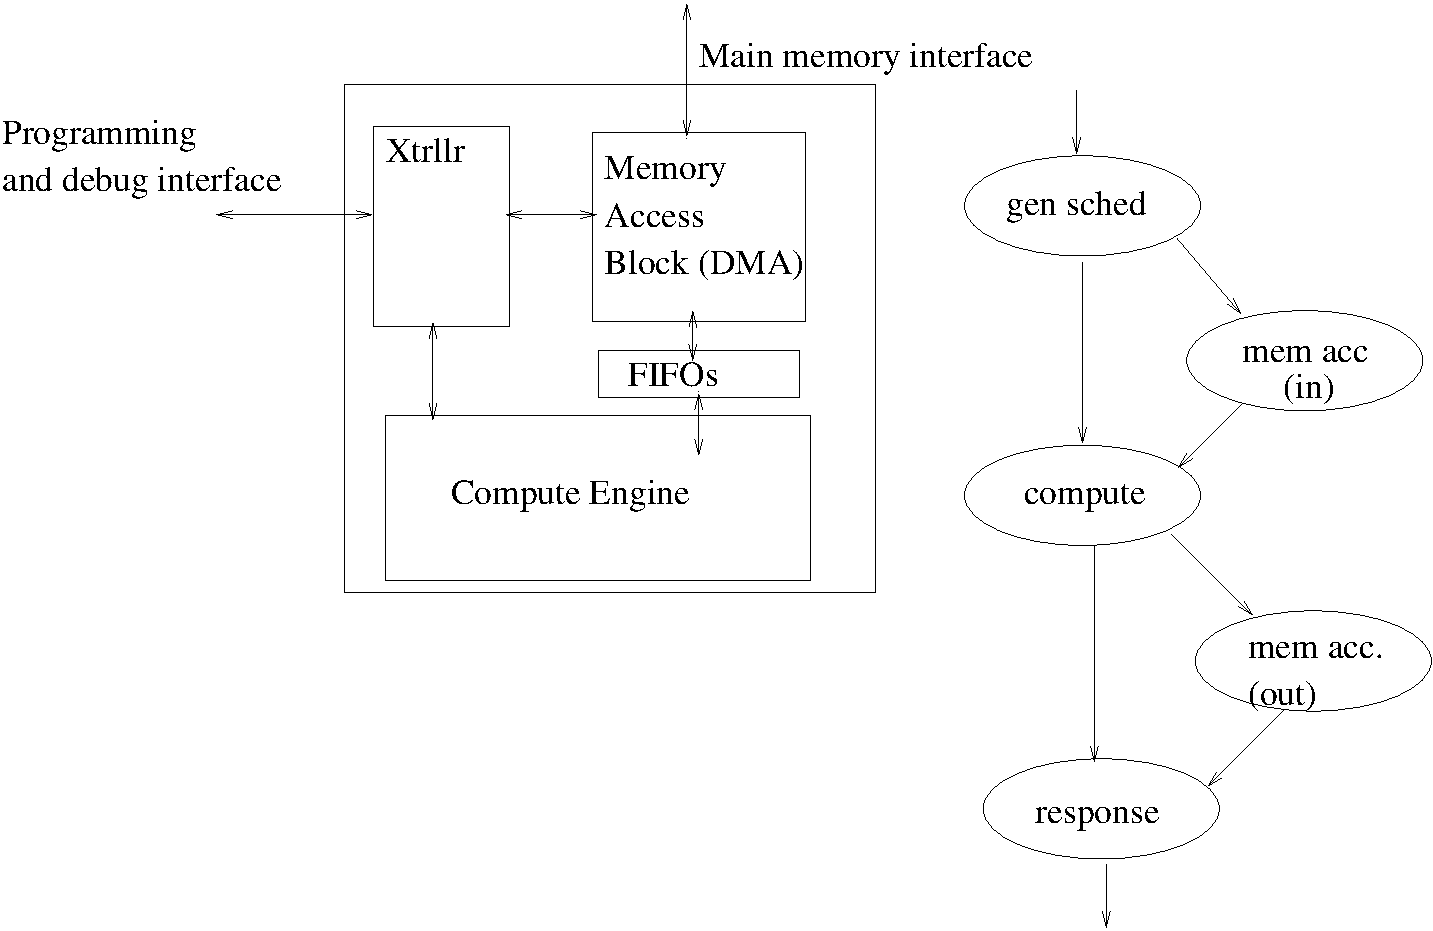
\includegraphics[width=10cm]{figs/UNET.pdf}
\caption{The UNET block diagram}
\label{fig:UnetBlockDiagram}
\end{figure}
}

\frame[containsverbatim]{\frametitle{NIC hardware implementation}
\begin{figure}
\centering
\includegraphics[width=10cm]{figs/NIC.pdf}
\caption{The NIC block diagram}
\label{fig:NicBlockDiagram}
\end{figure}
}

\frame[containsverbatim]{\frametitle{Demonstration setup}
\begin{figure}
\centering
\includegraphics[width=10cm]{figs/DemoBlockDiagram.pdf}
\caption{Demonstration Setup}
\label{fig:DemoSetup}
\end{figure}
}

\frame[containsverbatim]{\frametitle{Demonstration}
\begin{itemize}
\item Setup photo.
\item Download processor code.
\item Download UNET parameters.
\item Download image.
\item Cycle through UNET steps.
\begin{itemize}
\item Full performance mode: end-to-end processing of an image.
\item Debug mode: upload data after each UNET step, and confirm correctness.
\end{itemize}
\item Upload segmentation, confirm correctness.
\end{itemize}
}

\frame[containsverbatim]{\frametitle{Performance parameters}

\begin{itemize}
\item Clock frequency: 100MHz for processor, 125MHz  accelerator + nic, 50 MHz for Xilinx URAM.
\item Hardware LUT/FF cost.
\begin{itemize}
\item Processor core.
\item NIC.
\item Accelerator. 
\item Total.
\end{itemize}
\item Time required to download processor program (measured on host laptop).
\item Time required to download UNET parameters (measured on host laptop).
\item Time requred to download UNET image (measured on host laptop).
\item Total time required to complete UNET steps (measured inside the SOC).
\item Round trip time for an image (measured on host laptop).
\end{itemize}
}

\frame[containsverbatim]{\frametitle{Planned}
\begin{itemize}
\item Use DRAM and run  entire system at 125MHz.
\item Incorporate multiple engines to increase throughput.
\item Increase memory bus width to reduce latencies.
\end{itemize}
}
\end{document}
